\documentclass[12pt]{report}
\usepackage[utf8]{inputenc}
\usepackage{hyperref}
\usepackage{graphicx}
\usepackage[a4paper, width=150mm]{geometry}
\usepackage{acro}
\usepackage{fancyhdr}
\usepackage{float}
\usepackage{calc}
\usepackage{xcolor}
\usepackage{listings}
\usepackage[format=plain,labelfont={bf,it},textfont=it]{caption}

\definecolor{dkgreen}{rgb}{0,0.6,0}
\definecolor{gray}{rgb}{0.5,0.5,0.5}
\definecolor{dkyellow}{rgb}{0.8, 0.47, 0.196}
\definecolor{bg}{rgb}{0.96,0.96,0.96}

\lstset{
  language=Python,
  aboveskip=5mm,
  belowskip=5mm,
  showstringspaces=false,
  columns=flexible,
  basicstyle=\ttfamily\footnotesize,
  morekeywords={None,assert,List,with,TypeError,KeyError,AssertionError,True,AttributeError},
  keywordstyle=\color{blue},
  emph={__init__,method,property,static,@staticmethod,@classmethod,@property},
  emphstyle=\color{dkyellow},
  commentstyle=\color{dkgreen},
  stringstyle=\color{dkgreen},
  breaklines=true,
  breakatwhitespace=false,
  tabsize=4,
  backgroundcolor=\color{bg}
}

% \usepackage[backend=biber]{biblatex}
% \addbibresource{references.bib}

\hypersetup{
  pdfauthor={Chiemerie Ezechukwu}
}

\pagestyle{fancy}
\fancyhead{}
\rhead{\itshape\nouppercase{\leftmark}}

\setlength{\parskip}{\baselineskip}
\setlength{\parindent}{0pt}
\renewcommand{\baselinestretch}{1.3}

\graphicspath{{images/}}

\def\signat#1#2{\parbox{\widthof{#2}}{\textbf{#1:}\par #2}}

\DeclareAcronym{saas}{
  short=SaaS,
  long=Software as a Service
}

\DeclareAcronym{pm}{
  short=PM,
  long=Project management
}

\DeclareAcronym{oop}{
  short=OOP,
  long=Object oriented programming
}

\DeclareAcronym{o2pm}{
  short=O2PM,
  long=Object oriented project management
}

\DeclareAcronym{wbs}{
  short=WBS,
  long=Work breakdown structure
}

\author{Chiemerie Ezechukwu}


\begin{document}
  \begin{titlepage}
  \begin{center}

    \LARGE
    \textbf{POLITECNICO DI TORINO}

    \vspace{0.5cm}
    \large
    Master's Degree in Engineering and Management

    \vspace{0.5cm}

    
\includegraphics[width=0.6\textwidth]{polito.png}

    \vspace{0.5cm}
    Master's Degree Thesis

    \vspace{1cm}

    \Large
    % \textbf{Applying Object Oriented methodologies to Project Management objects and processes (Python).}
    \textbf{Design and Implementation of an Object-Oriented Python Library for Project Management}

    \vspace{1.5cm}

    \large
    \signat{Supervisor}{Prof. Demagistris Paolo Eugenio}
    \hfill
    \signat{Candidate}{Chiemerie Ezechukwu}

    \vfill

    Academic Year 2021/2022

  \end{center}
\end{titlepage}

  \chapter*{Abstract}
  \thispagestyle{plain}

When developing Project management backends, one often must plan for data types, ways to process the data and actions to take. This thesis explores how OOP methodologies benefit project management systems and software when the building blocks of the software or system are represented in terms of “self-sufficient” objects.

To improve the ease and speed with which applications are developed, there is the need for pre-developed libraries or framework. As such, a lot is abstracted from the library consumer, and they can come up with solutions quicker. A project management application is no exception to this and can benefit from a library that already implements or provides an interface for most project management objects and processes to be represented in the form of objects.

This thesis will produce a python library that models project management objects and processes that will be essential when developing a Python-based thesis project management application. For example, in a thesis setting, objects can be created to represent the project charter, the student involved, the professor and any other external stakeholders etc. These building blocks can then be aggregated, according to requirements, to form the core of the given project which should be self-sufficient (i.e., implement all the methods and attributes necessary). The benefits this will provide are many folds from appropriating the benefits of \acs{oop} to \acs{pm} to reduced efforts in the development process due to code reusability to increased flexibility due to modularity and polymorphism.

  \addcontentsline{toc}{chapter}{Abstract}

  \renewcommand{\contentsname}{Table of Contents}
  \setlength{\parskip}{0pt}
  \tableofcontents
  % \listoftables
  \listoffigures
  \printacronyms

  \setlength{\parskip}{\baselineskip}

  \chapter{Introduction}
  \section{Object oriented project management}
\subsection{What is project management}
Project management is the use of specific knowledge, skills, tools and techniques to deliver something of value to people \cite{pmi}.

Project management is the discipline of initiating, planning, executing, controlling and closing the work of a team to achieve specific goals and meet specific success criteria. A project is temporary in that it has a defined beginning and end in time, and therefore defined scope and resources \cite{harelimana}.

\subsection{What is a project}
A project, on the other hand, is distinct in that it is not a routine action, but rather a specific group of operations aimed at achieving a single goal. As a result, a project team frequently consists of people who don't normally collaborate - perhaps from separate businesses and across several continents. Examples of projects can be the creation of software to improve a corporate process, the construction of a building or bridge, the relief effort following a natural disaster, expansion into a new geographical market.

\subsection{Object oriented project management}
\ac{o2pm} is based on concepts of Object oriented programming such as objects and attributes, classes and members. It consists of five major activities;

\begin{itemize}
\item finding classes and objects.
\item identifying structures.
\item identifying subjects.
\item defining attributes.
\item defining services.
\end{itemize}

Most importantly, \ac{o2pm} is all about applying the object-oriented approach to project management \cite{chandrashekar}.

Coming from the standpoint of \ac{o2pm}, every aspect of a project is an object. In a typical project setting, the project manager constructs a project plan using a tool, defines tasks, dates, and effort, and assigns them to team members; however there are possibly no adequate mechanisms to encapsulate work and define boundaries. This often will lead to accountability issues, challenges with effectively quantifying project milestones and producing inaccurate reports.

Many of these issues are addressed by \ac{o2pm}. The object-oriented approach to project management is the focus of O2PM, and the key characteristics are as follows:

\begin{itemize}
  \item \textbf{Encapsulation:} Team members can work well within defined bounds when work deliverables are encapsulated meaning that boundaries are well defined. Better control and, more crucially, accountability will result from this type of job encapsulation. It also aids in the easy identification of issues and their resolution.
  \item \textbf{Inheritance:} will specify the project's architecture, rules, standards, and processes, which must be “inherited” by all team members and their work deliverables.
  \item \textbf{Polymorphism:} Describes the concept that a singular object/interface can have several other implementations. For example, in a thesis project, the professor and student are different entities but both implement the same stakeholder class.
  \item \textbf{Communication:} This defines a known and standard medium through which each encapsulated work object communicates with each other.
\end{itemize}

\section{Object oriented programming}
\subsection{What is Object oriented programming}
\acl{oop} (\acs{oop}) is a programming paradigm that relies on the concept of classes and objects. It is used to structure a software program into simple, reusable pieces of code blueprints (called classes), which are used to create individual instances of objects. There are many object-oriented programming languages including JavaScript, C++, Java, and Python to name a few \cite{educative}.

\ac{oop} allows programmers to handle software development as if they were dealing with actual real-world objects. People, in everyday life, have the knowledge and ability to do a variety of duties. Objects in OOP have fields to hold knowledge, state, and data, as well as the ability to execute numerous methods.

A class in \ac{oop} serves as a blueprint for creating more specific objects. They represent broad categories that share attributes. They enforce what attributes their instances can have but the values for any specific instance is set by that instance itself. For example, in project management, a stakeholder is a party who has an interest in a specific activity and can either affect or be affected by the said activity. Now there are several types of stakeholders but in the OOP world, they are all different implementation of the parent class/blueprint, stakeholder. In order words, any specific type of stakeholder, will be represented as an object, which itself is a specific example of the rather generic class, stakeholder and will have unique values to the properties defined in the class.
\begin{figure}[h]
  \centering
  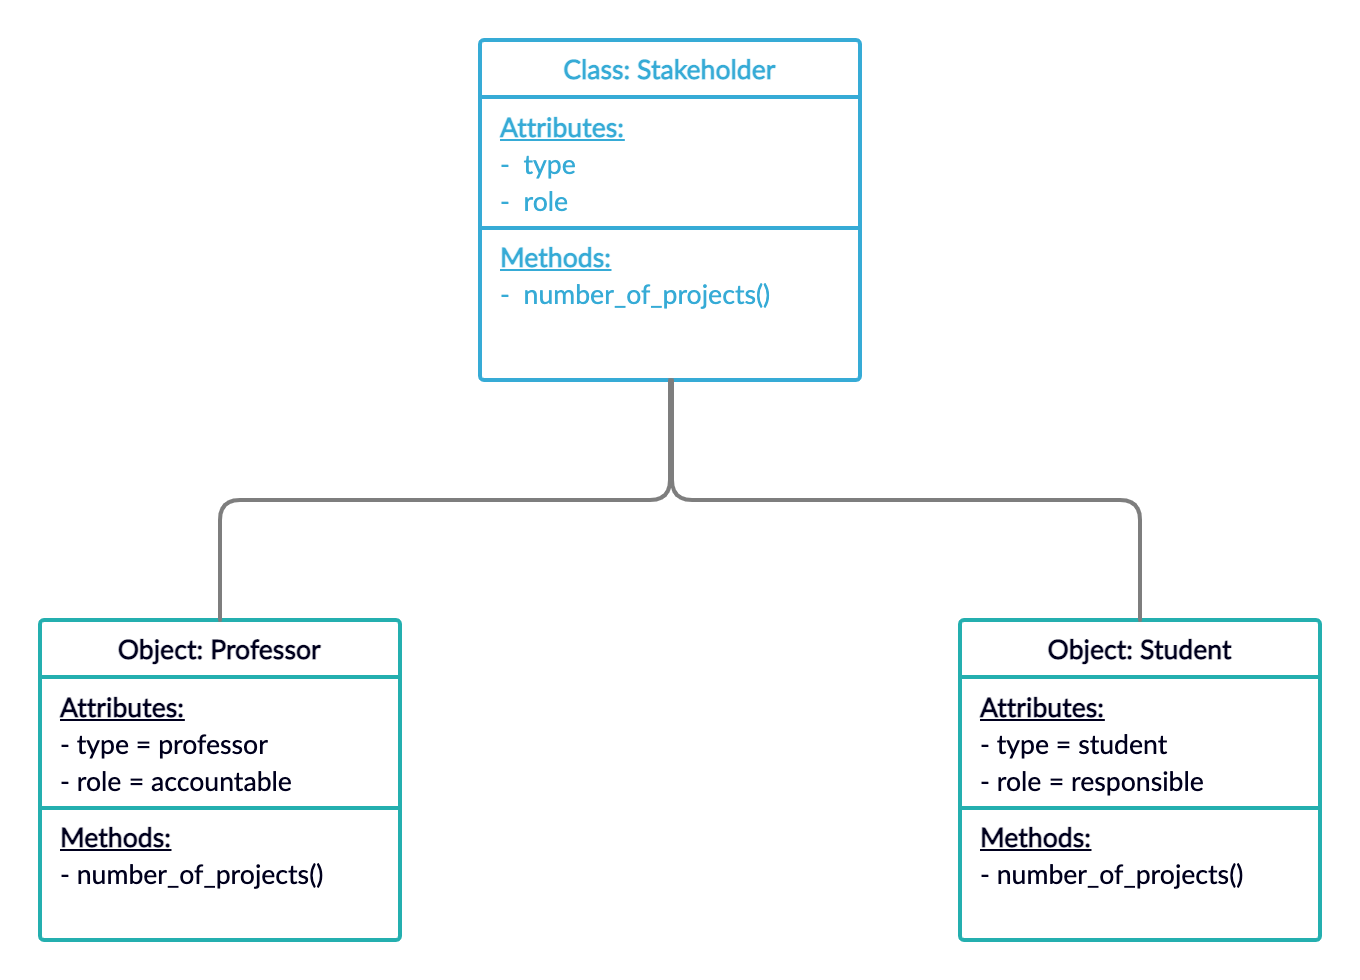
\includegraphics[width=130mm]{oop_illustration.png}
  \caption{Class Stakeholder implemented in Professor and Student class}
  \label{class blueprint}
\end{figure}

The above illustration visually depicts what has been explained so far. A Stakeholder class to contain all the properties a stakeholder must have and then from it are derived instances of a Stakeholder type object, Professor and Student to represent very specific stakeholders. Their attributes are isolated one from another and can be modified without affecting the original class or other objects. This means that the singular blueprint, Stakeholder can be reused to represent any number of stakeholders. The “role” field in the image above is according to RACI model which describes a responsibility assignment matrix.

The benefits that \acs{oop} presents are manyfold, from modelling complex things as simple reproducible structures to implementing objects that can be reused across programs to modifying the behavior of specific objects through polymorphism to their ability to protect information due to encapsulation.
It will be beneficial to explain some basic terminologies in OOP in the next section.

\subsection{Building blocks of OOP}
This section deals with elucidating the basic building blocks of an \acs{oop} program.

\subsubsection{Classes}
Classes are user-defined data types which is where the blueprint for the structure of attributes and methods are created. Individual objects can then be created or instantiated from this blueprint.

Classes have fields to hold attribute values and methods to model behavior. To illustrate, below is a code snippet in Python demonstrating how a generic class, \verb+Cat+ can be represented.
\begin{figure}[h]
  \centering
  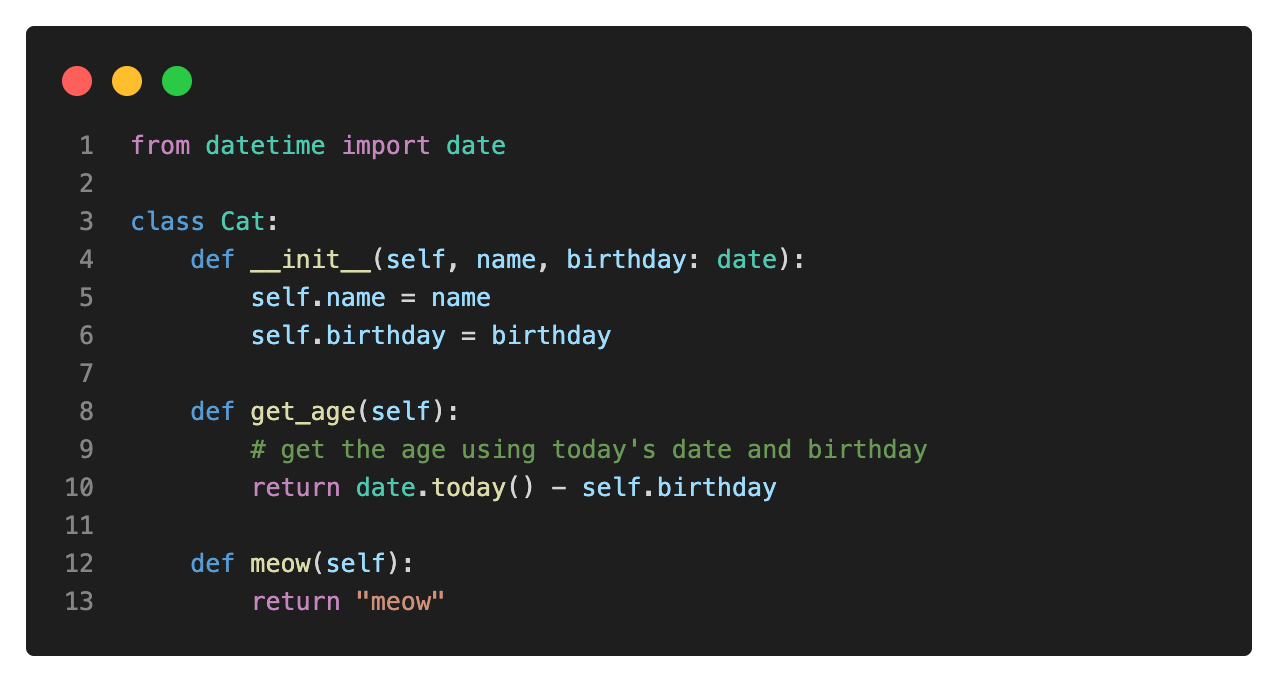
\includegraphics[width=130mm]{cat-code-snapshot.png}
  \caption{Cat class blueprint implementation}
  \label{cat class blueprint}
\end{figure}

The \verb+Cat+ class has attributes \verb+name+ and \verb+birthday+ and methods \verb+get_age()+ \verb+and meow()+.
With the knowledge that the class is only a blueprint for modelling a cat, a cat object can be instantiated from it to represent an individual real-world thing.

\subsubsection{Objects}
\ac{oop} is all about objects. Objects are instances of a class created with specific data. In code snippet, \verb+milana+ is an instance of the \verb+Cat+ class
\begin{figure}[h]
  \centering
  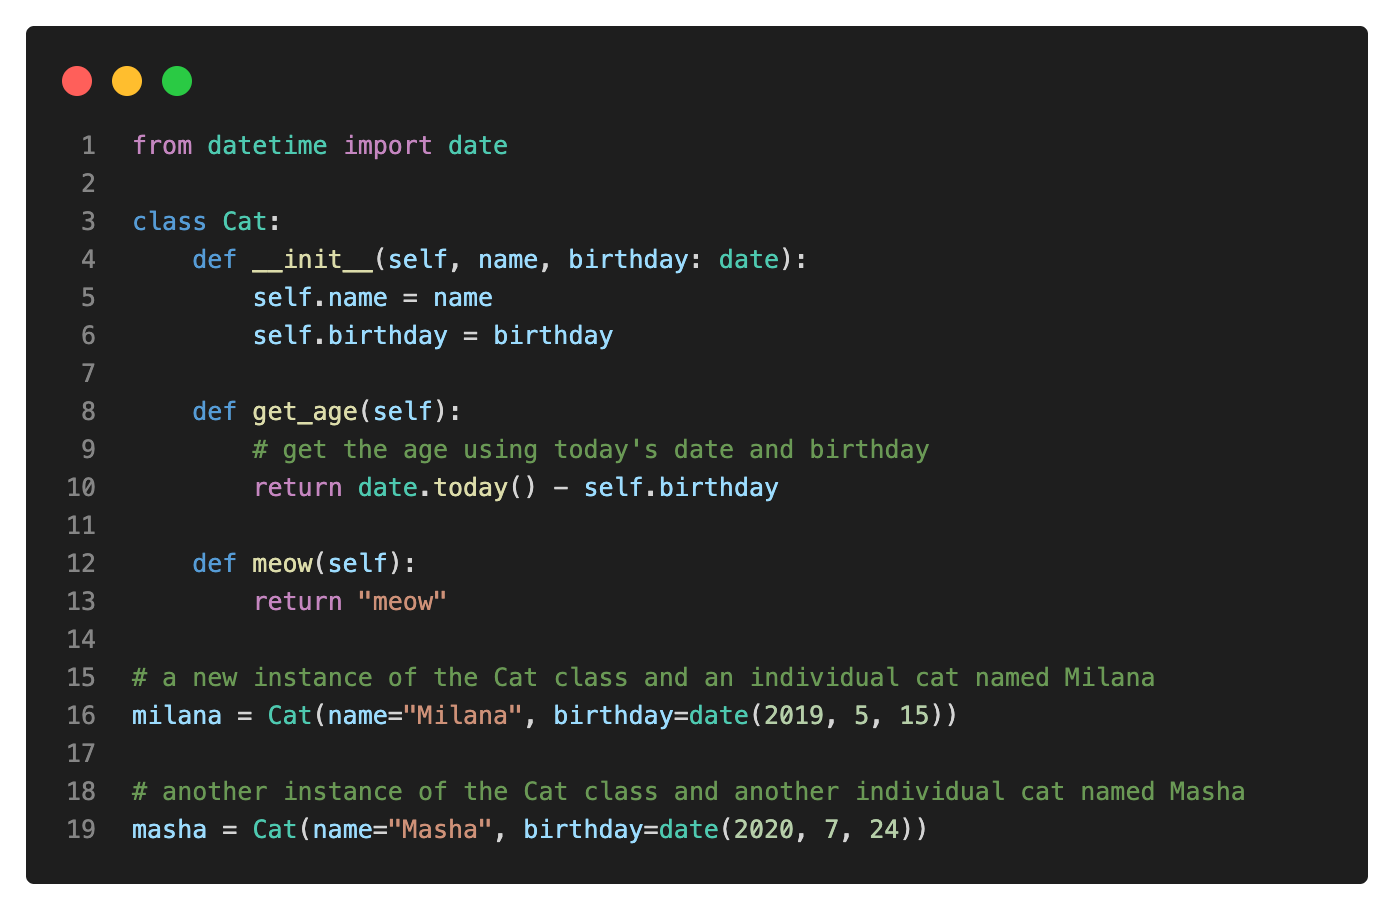
\includegraphics[width=130mm]{cat-instance-code-snapshot.png}
  \caption{Cat class instance}
  \label{cat class instance}
\end{figure}

When the \verb+Cat+ class is called like on lines 16 and 19:

\begin{itemize}
  \item A new object is created each time and stored in the variables \verb+milana+ and \verb+masha+ respectively.
  \item The constructor (\verb+__init__+) method runs with the \verb+name+ and \verb+birthday+ arguments and assigns values.
\end{itemize}

\subsubsection{Attributes}
The information that is stored is referred to as attributes. The Class template defines the attributes. Individual objects have data stored in the attributes field when they are instantiated.

The data in the object's attributes fields define the object's state. The \verb+birthday+ attribute could define the state of an object, allowing software to manage cats of various ages differently.

\subsubsection{Methods}
The behaviors of objects are represented by methods. Methods carry out operations, such as returning information about an object or updating its data. The code for the method is specified in the class definition.

Objects can invoke the methods described in the class when they are instantiated. In the code snippet below, the \verb+meow()+ method is defined in the \verb+Cat+ class and the \verb+meow()+ method is called on either the \verb+milana+ or \verb+masha+ object on lines 21 and 22 respectively.
\begin{figure}[h]
  \centering
  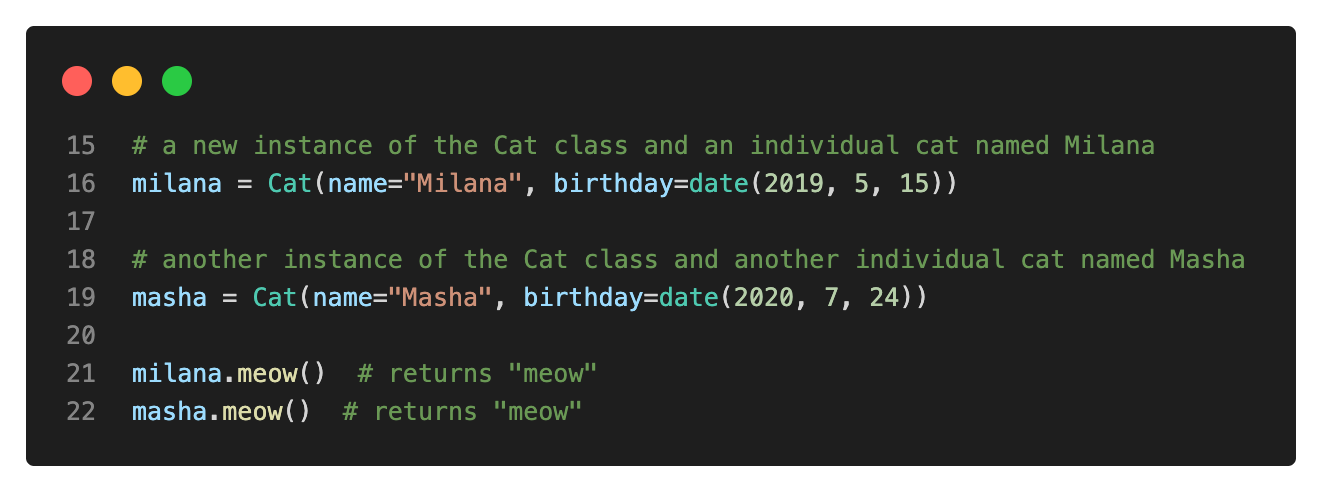
\includegraphics[width=130mm]{cat-instance-methods-code-snapshot.png}
  \caption{class methods}
  \label{cat class methods}
\end{figure}

Methods are often employed to modify, update or delete data but they don’t have to. As a matter of fact, the \verb+meow()+ method does not modify any data because meowing does not modify any of the attributes of the \verb+Cat+ class, \verb+name+ or \verb+birthday+.
Methods are how programmers keep functionality encapsulated within an object and promote reusability. When debugging, its reusability comes in handy. If an error occurs, there is only one location to look for it and correct it rather than numerous.

\section{Principles of \acs{oop}}
There are four main pillars of \acs{oop};
\begin{itemize}
  \item \textbf{Inheritance:} Child classes inherit data and behavior from their parent classes.
  \item \textbf{Encapsulation:} The process of enclosing information in an object and exposing only a necessary subset.
  \item \textbf{Abstraction:} exposing high-level public methods for accessing an object.
  \item \textbf{Polymorphism:} many methods can do the same task.
\end{itemize}

\subsubsection{Inheritance}
Objects typically have a lot in common. They have some similar logic. However, they are not comparable. Inheritance allows to reuse the common logic and extract the unique logic into another separate class. It implies that a (child) class can be created by deriving from another (parent) class. The child class derives all the parent class's fields and methods (common part) and can implement its own (unique part).

Herding dogs, for example, have a one-of-a-kind capacity to herd animals. To put it another way, all herding dogs are dogs, but not all dogs are herding dogs. This distinction can be illustrated by establishing a \verb+HerdingDog+ child class from a parent \verb+Dog+ class, and then adding the unique \verb+herd()+ behavior to it.

Inheritance has the advantage of allowing programs to build a generic parent class and then create more specific child classes as needed. This simplifies the overall development because, rather than duplicating the \verb+Dog+ class's structure repeatedly, child classes can have automatic access to their parent class's features.
\begin{figure}[H]
  \centering
  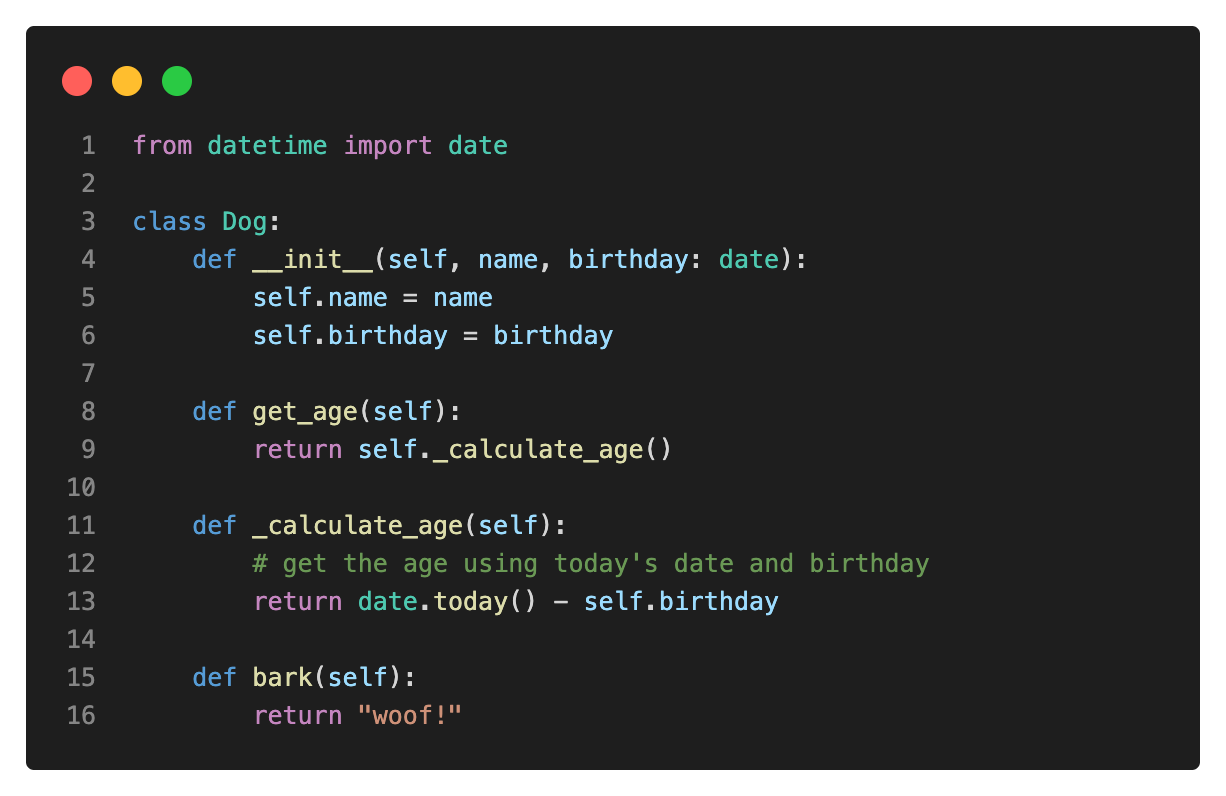
\includegraphics[width=130mm]{dog-code-snapshot.png}
  \caption{Generic Dog class}
  \label{generic dog class}
\end{figure}

In the code snippet in \autoref{inheritance illustration}, the child class \verb+HerdingDog+ inherits the method bark from the parent class \verb+Dog+ in \autoref{generic dog class} and adds a new method \verb+herd()+.
\begin{figure}[H]
  \centering
  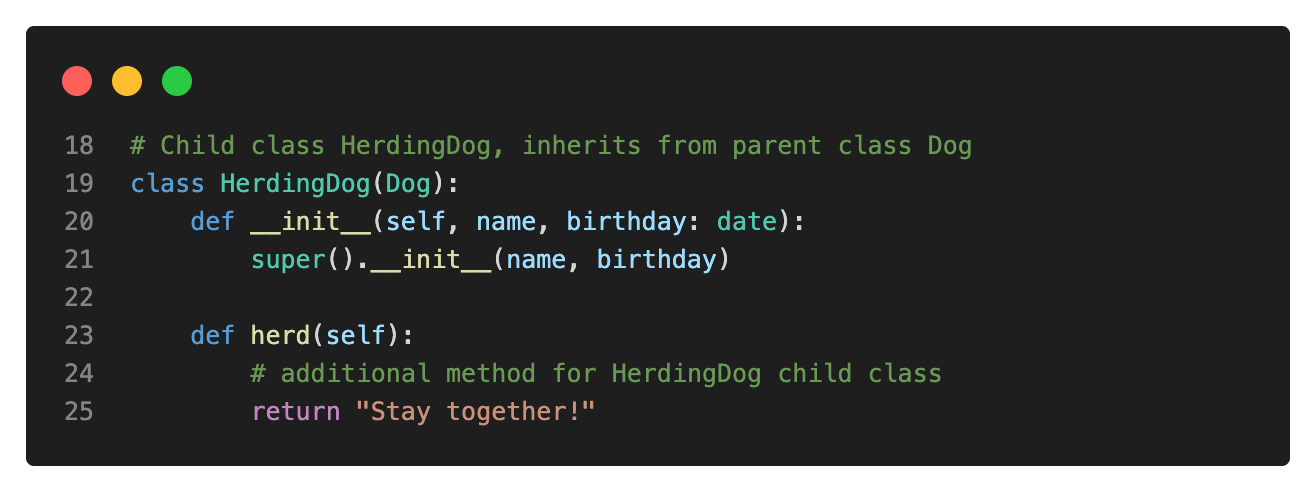
\includegraphics[width=130mm]{herd-dog-code-snapshot.png}
  \caption{Inheritance illustration}
  \label{inheritance illustration}
\end{figure}

The \verb+bark()+ method is not duplicated in the \verb+HerdingDog+ class; instead, it inherits the \verb+bark()+ method defined in the parent \verb+Dog+ class defined in \autoref{generic dog class}.

\begin{figure}[H]
  \centering
  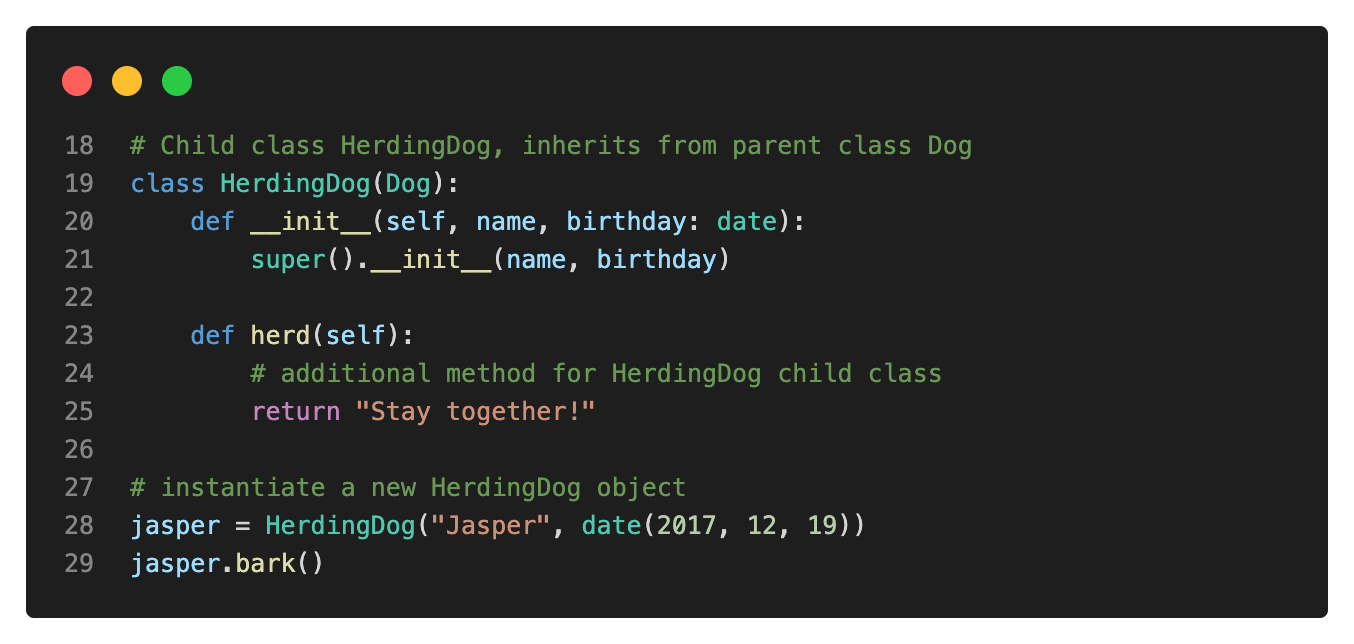
\includegraphics[width=130mm]{herd-dog-instance-code-snapshot.png}
  \caption{Child class instance}
  \label{child class instance}
\end{figure}

When the code in \autoref{cat class instance} calls \verb+jasper.bark()+ method, the \verb+bark()+ method traverses up the chain to the parent where the method has been defined.

\subsubsection{Encapsulation}
Encapsulation is the process of enclosing all critical information within an object and only presenting part of it to the outside world. Code within the class template defines attributes and behaviors.

Encapsulation hides the internal software code implementation inside a class and hides internal data of inside objects.

Encapsulation is achieved when each object keeps its state private, inside a class. Other objects don’t have direct access to this state. Instead, they can only call a list of public methods.

As an example of encapsulation, consider an automobile. Public interfaces are how the automobile communicates with the outside world by employing blinkers to signal turns. Under the hood, on the other hand, the engine is hidden.

Security is improved via encapsulation. Private attributes and methods can be defined to prevent access from outside the class. Public methods and properties are used to obtain or alter data in an object.

Using the \verb+Dog+ class example, encapsulation helps here so that access to private information on other \verb+Dog+ instances is not possible. Consider the \verb+get_age()+ method in \autoref{generic dog class}, the calculation is hidden inside the \verb+Dog+ class and each instance of the class will use the \verb+get_age()+ method to access the \verb+age+ data. Since methods can also update an object’s data, the developer controls what values can be changed through public methods.

\subsubsection{Abstraction}
Abstraction can be thought of as a natural extension of encapsulation. It refers to the user's interaction with only a subset of an object's attributes and operations. To access a complex object, abstraction use simplified, high-level tools. When employing abstraction, each object should only disclose a high-level mechanism for interacting with it. Internal implementation details should be hidden behind this mechanism. Using the automobile example again, you don’t have to know the details of the inner workings of the engine to drive it. The driver utilizes only a few tools, such as the gas pedal, brake, steering wheel, and blinker. The driver is not privy to the engineering. A lot of elements must function together under the hood to make an automobile run but revealing that knowledge to the driver would be a risky distraction.

In the \verb+Dog+ class example in \autoref{generic dog class}, the calculation of the age has been abstracted away into a private method \verb+_calculate_age()+ and a simple public method \verb+get_age()+ is exposed as a way to get the age information

The benefits of abstraction are summarized below:
\begin{itemize}
  \item Simple, high level user interfaces.
  \item Complex code is hidden.
  \item Security.
  \item Easier software maintenance.
  \item Updates to code will rarely change abstraction.
\end{itemize}

\subsubsection{Polymorphism}
Polymorphism refers to the design of items that have similar behavior. Objects can override shared parent behaviors with specific child behaviors through inheritance. Method overriding and method overloading are two ways that polymorphism allows the same method to perform various actions.

\begin{itemize}
  \item \textbf{Method Overriding} \\ In method overriding, the child class will provide its own implementation of a method already in the parent class effectively overriding it. If for the \verb+Dog+ class, there’s the need to create another child class \verb+TrackingDog+ which for some reason barks differently, the \verb+bark()+ method established in the parent class will have to be overridden like in the code snippet in \autoref{method overriding} to produce a different bark sound.

  \item \textbf{Method Overloading} \\ This kind of polymorphism happens at compile or code execution time. Methods may have the same name but behave differently based on the number of parameters passed to them.

  \begin{figure}[H]
    \centering
    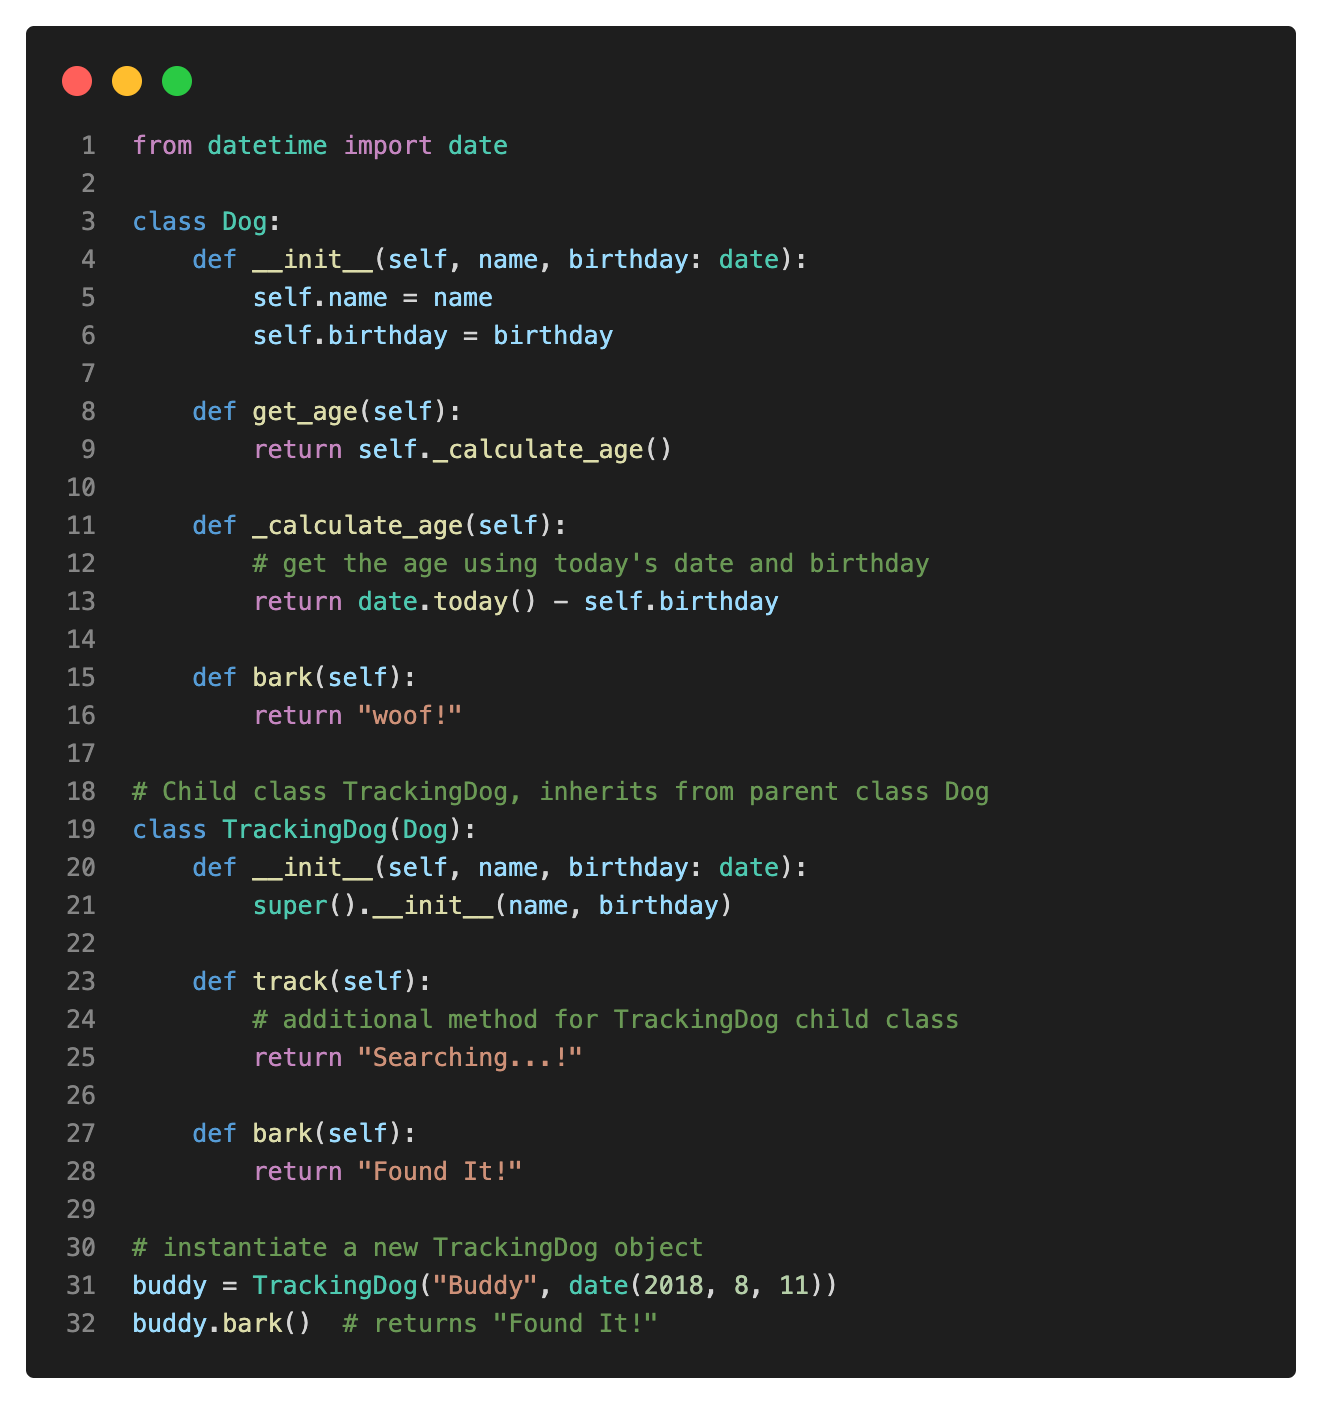
\includegraphics[width=130mm]{track-dog-overriding-instance-code-snapshot.png}
    \caption{Method overriding}
    \label{method overriding}
  \end{figure}
\end{itemize}

The benefits of Polymorphism are:

\begin{itemize}
  \item Objects of different types can be passed through the same interface.
  \item Method overriding.
  \item Method overloading.
\end{itemize}

\section{Libraries}
A "library" is a collection of program parts that do common and/or specialized things that save the programmer from needing to "reinvent the wheel" when writing software. A class library is a pre-coded OOP template collection. It usually consists of functions to call and object classes you can instantiate \cite{stevenparker}.

Libraries encourage code reuse and decrease redundancy by providing implementation of repetitive jobs.  Developing programs from the ground up can be a time-consuming and costly task. Class libraries include all necessary classes in a previously written coded format, making programming easier while also improving code quality. Customizing the class template is done in accordance with the programming requirements. To minimize programming language limitations, class libraries are regularly updated, and time verified for stability.

Programmers can decide to build everything from the ground up, but this is incredibly unsustainable and ill-advised for the reasons below;

\begin{itemize}
  \item \textbf{Expertise in the domain covered by the library:} Authors are usually experts in the domain covered by the library. This will ensure that users of the library get the best implementation possible.
  \item \textbf{Stability:} Libraries have the benefit of being used by hundreds, if not thousands, of developers around the world. Most of the early issues have already been encountered and resolved by authors.
  \item \textbf{Knowledge:} By having to use code pre-written by others, developers gain knowledge in the process. Many well-known libraries are built by top developers and serve as excellent examples of solid coding and design.
  \item \textbf{Finances:} For commercial libraries, the equivalent of hundreds, if not thousands, of man days of work can be got for free thanks to open source.
\end{itemize}

\section{Overview of the thesis}
This thesis project takes a practical approach at implementing a library that can be used when making

  \chapter{Implementation}
  The implementation of this thesis project focuses on the library to be developed with the Python programming language.
\section{Tools and technologies used}
\subsection{Python}
Python is a programming language that is commonly used to create websites (server-side) and applications, automate operations, and perform data analysis. Python is a general-purpose programming language, which means that it can be used to develop a wide range of applications and isn't specialized for any particular problem. Because of its versatility and beginner-friendliness, it has become one of the most widely used programming languages today.

Python was designed for readability and has some similarities to the English language with influence from mathematics. Python relies on indentation, using whitespace, to define scope; such as the scope of loops, functions and classes. Other programming languages often use curly braces for this purpose.

Python is popular for a variety of reasons from its simple syntax that mimics natural language to its versatility to the large and incredibly active community that contributes to Python’s pool of modules and libraries.

\subsection{Git and GitHub (Version Control)}
\subsubsection{Git}
From web developers to app developers, Git is useful to anyone who writes code or track changes to files. Git is the most used version control system. It keeps track of the changes you make to files so you can see what has been done and go back to previous versions if you need to. Git also facilitates cooperation by allowing several people's modifications to be merged into a single source. Initialize Git locally and your files and their history are stored on your computer. Git repositories contains all the project files and the entire revision history. It can be created by running the \verb+git init+ command in the location you wish to create this repository. This creates a \verb+.git+ subfolder, which contains all of the Git metadata for tracking changes.

\subsubsection{GitHub}
GitHub, on the other hand, is a Git hosting repository that makes it easier for developers to work together. Developers can work on the same code repository without conflicts using features like pull requests, code review, and issues (ticketing system).

Developers can work on separate branches of the same repository, commit code changes to store them, create a pull request to the main branch, debate and peer-review code changes before merging the pull request.

A repository is sometimes known as a repo. Repos are Git projects that contain files and directories associated with a development project, as well as the revision history of each file. Within a repository, new branches can be created, pull requests can be made, and merges can take place. The changelog displays the history of file changes in the repository.

Git and GitHub has been employed to store and version all code modifications for this project.

\subsubsection{Why use Git}
\begin{itemize}
  \item \textbf{Simplifies the process of contributing to open source:} GitHub is used by nearly every open-source project to administer their project. If your project is open source, GitHub is free to use, and it contains a wiki and issue tracker that makes it simple to provide more detailed documentation and receive feedback. To contribute, simply fork a project, make your changes, and submit a pull request via the GitHub web interface.
  \item \textbf{Documentation:} You make it easy to get quality documentation by using GitHub. They include articles on practically every issue related to git that you can think of in their help section and tutorials.
  \item \textbf{Showcase your work:} Do you want to attract recruiters as a developer? The finest tool you can use for this is GitHub. Most firms now check at GitHub profiles while looking for fresh hires for their projects. Even if you did not attend a prestigious university or college, if your profile is available, you will have a better chance of being hired.
  \item \textbf{Markdown:} Markdown allows you to write styled texts using a simple text editor. Everything on GitHub is written in Markdown, including the issue tracker, user comments, and everything else. With so many other computer languages to master in order to build up projects, having your content inputted in a format without having to learn yet another system is a huge benefit.
  \item \textbf{Repository} This has previously been noted, but it's worth repeating: GitHub is a repository. This means that it is possible for your work to be seen by the general audience. Furthermore, GitHub is one of the largest coding communities in the world right now, giving your project a lot of exposure.
  \item \textbf{Keep track of changes in your code over time:} It's difficult to maintain track of modifications when numerous people work on a project—who modified what, when, and where those files are stored. This problem is solved by GitHub, which keeps track of all the modifications that have been pushed to the repository. You can keep a version history of your code, much like you can with Microsoft Word or Google Drive, so that earlier versions aren't lost with each iteration.
  \item \textbf{Options for integration:} GitHub integrates with popular cloud platforms like Amazon and Google Cloud, as well as feedback tracking services like Code Climate, and can highlight syntax in over 200 different programming languages.
\end{itemize}

\subsection{GitHub Actions}
For continuous integration (CI), GitHub Actions has been employed.

GitHub Actions is a continuous integration and continuous delivery (CI/CD) platform that allows you to automate your build, test, and deployment pipeline. It allows for creating workflows that build and test your source code on events you configure happening in your repository like pull requests or even merge pull requests to production \cite{githubactions}.

GitHub Actions extends beyond DevOps by allowing you to execute workflows in response to other events in your repository. For example, anytime someone opens a new issue in your repository, you may execute a workflow to automatically add the required labels.

You can execute your workflows on GitHub's virtual machines running Linux, Windows, and macOS, or you can host your own self-hosted runners in your own data center or cloud infrastructure.

\subsubsection{The components of GitHub Actions}
When an event occurs in your repository, such as when a pull request is opened or an issue is raised, you may set up a GitHub Actions workflow to be executed. Your workflow includes one or more jobs that can execute sequentially or concurrently. Each task contains one or more steps that either run a script you create or run an action, which is a reusable addition that can streamline your workflow.

\begin{figure}[H]
  \centering
  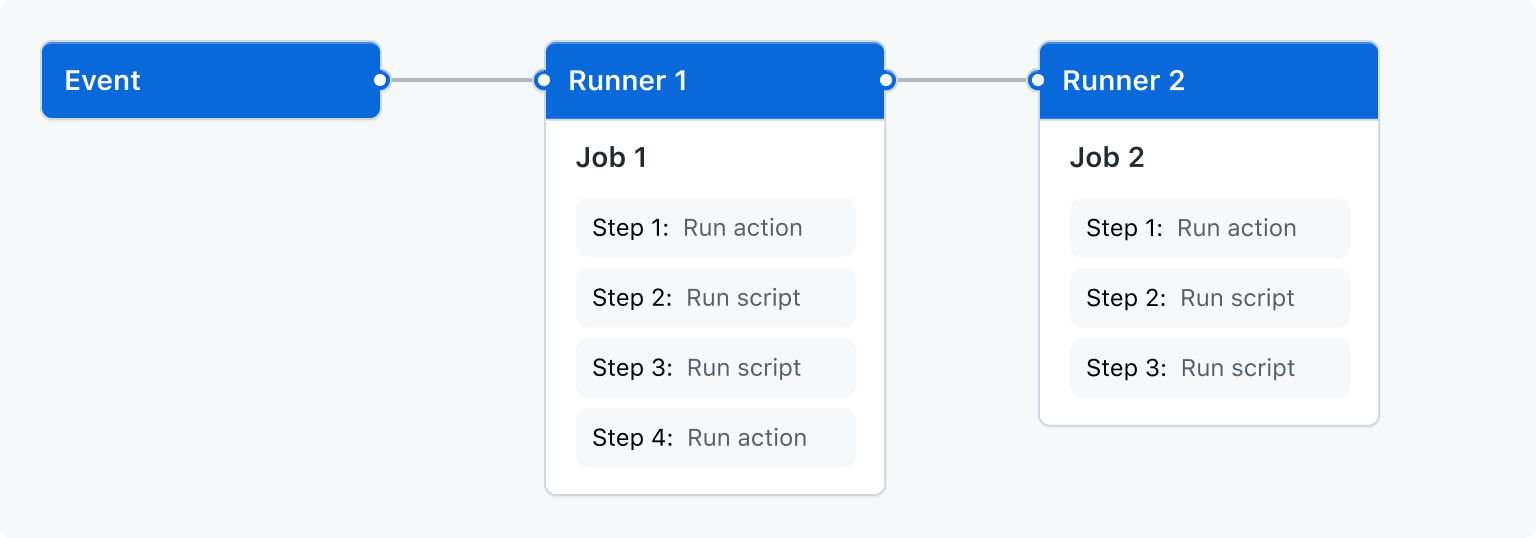
\includegraphics[width=130mm]{overview-github-actions.png}
  \caption[Components of GitHub Actions]{Components of GitHub Actions \cite{githubactions}}
  \label{github actions}
\end{figure}

\subsubsection{Workflows}
A workflow is a programmable automated procedure that executes one or more tasks. Workflows are specified in a YAML file that is checked into your repository. They can be triggered by an event in your repository, manually, or on a set timetable.

A repository can contain numerous workflows, each of which can carry out a separate set of tasks. For example, you may have one workflow to build and test pull requests, another to deploy your application whenever a release is made, and still another to add a label if someone reports a new issue.

\subsubsection{Events}
A workflow run is triggered by an event, which is a specific activity in a repository. For example, GitHub can be an activity when someone creates a pull request, opens an issue, or pushes a commit to a repository. A workflow can also be started manually on a timetable, or by triggering a REST API.

\subsubsection{Jobs}
A job is a series of workflow stages that all run on the same runner. Each step consists of either a shell script that will be run or an action that will be performed. The steps are carried out in a sequential order and are interdependent. Because each step is run on the same runner, data can be shared from one step to the next. A step that builds your application, for example, could be followed by a step that tests the application that was built.

You can configure a job's dependencies with other jobs; by default, jobs execute in parallel and have no dependencies. When a job becomes reliant on another job, it will not run until the dependent job has completed. You might have many build tasks for different architectures with no dependencies and a packaging job that is dependent on those jobs, for example. The build jobs will run in parallel, and the packaging job will begin once they have all completed successfully.

\subsubsection{Actions}
An action is a GitHub Actions platform custom application that performs a sophisticated but regularly repeated activity. To assist in limiting the amount of repetitive code in your workflow files, use an action. An action can grab your git repository from GitHub, configure your build environment's toolchain, or set up your cloud provider's credentials.

\subsubsection{Runners}
When your workflows are triggered, a runner is a server that executes them. Each runner is limited to one job at a time. To run your workflows, GitHub provides Ubuntu Linux, Microsoft Windows, and macOS runners; each workflow run takes place in a new, freshly provisioned virtual machine. You can host your own runners if you need a different operating system or a specific hardware setup.

\section{Library Implementation}
In this section, the implementation of the library is showcased and explained. The library will have 8 distinct project management objects each represented as a class in the library namely;

\begin{itemize}
  \item \verb +ProjectCharter+ class
  \item \verb +Stakeholder+ class
  \item \verb +Deliverable+ class
  \item \verb +ProjectGovernance+ class
  \item \verb +Risk+ class
  \item \verb +WBSItem+ class
  \item \verb +WBS+ class
  \item \verb +Project+ class
\end{itemize}

\subsection{The ProjectCharter class}
A project charter is a formal, typically short document that describes your project in its entirety — including what the objectives are, how it will be carried out, and who the stakeholders are. It is a crucial ingredient in planning the project because it is used throughout the project lifecycle \cite{wrike}.

The \verb+ProjectCharter+ class presents a few methods and properties.

The class's methods and signatures are represented below in a very simplified interface to abstract away the implementation.\\
\begin{lstlisting}
  class ProjectCharter(project_title = None):
      # properties
      property executive_summary: str
      property project_stakeholders: list
      property project_title: str

      # methods
      method add_stakeholder(self, stakeholder)

      # static methods
      static is_class_stakeholder(obj) -> bool
\end{lstlisting}

The constructor is called anytime a new \verb+ProjectCharter+ instance is created. It takes an optional argument, \verb+project_title+ and goes ahead to initialize an empty list \verb+_project_stakeholders+ private property that will hold and track \verb+Stakeholder+ objects

The \verb+executive_summary+ property is a string field that holds summarized information about project.

There's a restriction to the \verb+ProjectCharter+ class in that only objects initialized from the \verb+Stakeholder+ class can be added to the \verb+project_stakeholders+ list. \linebreak Adding a stakeholder must be done through the method \verb+add_stakeholder+. A static method \verb+is_class_stakeholder+ is available solely for verifying objects before they are accepted to the stakeholder list. The static method simple returns a boolean \verb+True+ or \verb+False+ and is used in the method \verb+add_stakeholder+ like below\\*

\begin{lstlisting}
  def add_stakeholder(self, stakeholder):
      assert self.is_class_stakeholder(stakeholder)
      if isinstance(stakeholder, (list, tuple)):
          for s in stakeholder:
              self.__finalize_add_stakeholder(s)
      else:
          self.__finalize_add_stakeholder(stakeholder)
\end{lstlisting}

\vfill

\begin{lstlisting}
  @staticmethod
  def is_class_stakeholder(obj) -> bool:
      """
      Checks that the stakeholder about to be added to the project
      is instance of the Stakeholder class
      """
      if isinstance(obj, list):
          return all(isinstance(s, Stakeholder) for s in obj)
      return isinstance(obj, Stakeholder)
\end{lstlisting}


\subsection{The Stakeholder class}
This class provides a template for modelling stakeholder objects. Its methods, properties and signatures are below in a simplified interface.

\begin{lstlisting}
  class Stakeholder(first_name, last_name, email):
      # methods
      method add_to_involved_projects(self, value)
      method get_full_name(self) -> str
      method get_number_of_projects(self) -> int

      # properties
      property projects_involved: List[Project]
      property responsibility: str
      property role
      property stakeholder_title
      property stakeholder_type
\end{lstlisting}

The method \verb+add_to_involved_projects+ is designed to be used only by the \linebreak \verb+__finalize_add_stakeholder()+ private method defined in the \verb+ProjectCharter+ class. It is simply used to add new \verb+ProjectCharter+ instances to the list of projects the stakeholder in question is involved with.

\verb+get_number_of_projects()+ simply returns an integer depicting the number of projects that stakeholder instance is involved with at any point in time.

The property \verb+projects_involved+ returns a list of objects of the \verb+ProjectCharter+ charter class readily available should the library consumer require it.

For the \verb+role+ property of the various stakeholders, a simple enum following the RACI responsibility models is defined.

\begin{lstlisting}
  class RoleEnum(Enum):
      """
      * R = Responsible (Those who do the work to complete the task)
      * A = Accountable (also approver or final approving authority)
      * C = Consulted (Those whose opinions are sought)
      * I = Informed (Those who are kept up-to-date on progress)
      """

      RESPONSIBLE = "R"
      ACCOUNTABLE = "A"
      CONSULTED = "C"
      INFORMED = "I"
      UNSET = "UNSET"
\end{lstlisting}


\subsection{The Deliverable class}
Deliverables are very important to the success of any project and this library provides an implementation of a deliverable model. The methods and properties it provides are showcased in the simple interface below

\begin{lstlisting}
  class Deliverable(doc_title):
      # methods
      method mark_as_accepted(self)
      method mark_as_rejected(self)
      method set_reviewer(self, value)

      # properties
      property accepted: bool
      property reviewer
      property acceptance_criteria
      property description
      property expected_result
\end{lstlisting}

The \verb+mark_as_accepted+ and \verb+mark_as_rejected+ methods serve to set the \verb+accepted+ property to \verb+True+ or \verb+False+ depending on whether the deliverable has been accepted or not. \verb+set_reviewer+ sets the \verb+reviewer+ property to the "responsible" who is accountable for the deliverable. \verb+acceptance_criteria+ property serves to define what determines when a deliverable can be accepted or not.


\subsection{The ProjectGovernance class}
Project Governance is the set of rules, procedures and policies that determine how projects are managed and overseen.

These rules and procedures define how decisions are made during projects. As part of the oversight process, project governance also determines the metrics by which project success is measured.

The methods and properties this class implements are in the simplified interface below.

\begin{lstlisting}
  class ProjectGovernance(project):
      # methods
      method get_all_stakeholders(self) -> list
      method sign_agreement(self, signee: Stakeholder)

      # properties
      property not_signed_by: list
      property signed_by: list
      property signed_by_all: bool
\end{lstlisting}

The \verb+get_all_stakeholders+ method simply returns a list of stakeholder objects included in the current project governance object.

\verb+sign_agreement+ simply exposes a method used to sign the project governance by the stakeholder object passed in the argument.

There are a few properties in this class as well. \verb+not_signed_by+ returns a list of stakeholder objects included in the project governance object but has yet to consent the terms that will govern the project execution. \verb+signed_by+ also returns a list of stakeholder objects and is the exact opposite of the former.
\verb+signed_by_all+ is a boolean type that simple returns \verb+True+ if all the involved stakeholders have signed and \verb+False+ otherwise.


\subsection{The Risk class}
Risk is any unexpected event that can affect your project — for better or for worse \cite{wrike-2}. People, processes, technology, and resources can all be impacted by risk. Risks are not the same as issues, which is a crucial distinction to recognize. Issues are something you know you'll have to deal with and may even know when they'll happen, such as a planned vacation for a team member or a large rise in product demand during the holidays. Risks are occurrences that can happen at any time and that you may not be able to predict — for example, a sudden outbreak of flu in your office or a critical product component being out of stock.

The \verb+Risk+ class for this library has an interface as showcased below

\begin{lstlisting}
  class Risk(risk_name, probability, impact)
      # methods
      method assign_risk_owner(self, value)
      method get_risk_score(self)
      method set_counter_measure(self, counter_measure)

      # properties
      property counter_measure
      property description
      property impact
      property probability
      property risk_owner
\end{lstlisting}

\verb+assign_risk_owner+ is simply the method for assigning the risk owner. \linebreak \verb+get_risk_score+ is a value calculated based on the \verb+probability+ and \verb+impact+ \linebreak properties. An Enum class \verb+RiskScore+ is defined to organize the various risk score points and is the return type of the method \verb+get_risk_score+.

\begin{lstlisting}
  class RiskScore(Enum):
      VERY_HIGH = range(80, 101)  # 80% - 100%
      HIGH = range(50, 80)  # 50% - 79%
      MODERATE = range(30, 50)  # 30% - 49%
      LOW = range(0, 30)  # 0 - 29%

      @classmethod
      def get_risk_score(cls, value):
          for val in cls:
              if value in val.value:
                  return val
\end{lstlisting}

The \verb+set_counter_measure+ method is responsible for setting the counter measure to be adopted for mitigating the particular risk object in question.

There are a possible of allowed values for the return value of the \verb+set_counter_measure+ method. It is defined in the \verb+RiskCounterMeasure+ Enum class

\begin{lstlisting}
  class RiskCounterMeasure(Enum):
      REDUCE = "REDUCE"
      PREVENT = "PREVENT"
      ACCEPT = "ACCEPT"
      TRANSFER = "TRANSFER"

      @classmethod
      def list_allowed_values(cls):
          return list(map(lambda c: c.value, cls))
\end{lstlisting}


\subsection{The WBS class}
The \ac{wbs} class provides an interface for organizing objects from the \verb+WBSItem+ class. The \verb+WBSItem+ class's properties are displayed below

\begin{lstlisting}
  class WBSItem(work_item_name, duration, lag):
      # properties
      property duration
      property lag
      property objective
      property percent_complete
      property resource
      property status
\end{lstlisting}

Several \verb+WBSItem+ objects are aggregated under a list type property to make up part of the \verb+WBS+ class.

Here is a look at the \verb+WBS+ class simplified interface

\begin{lstlisting}
  class WBS(name, start_date):
      # methods
      method add_wbs_item(self, *args: WBSItem)
      method get_critical_path(self)
      method link_nodes(self, *args: Tuple[WBSItem, WBSItem])
      method update_all(self)

      # properties
      property duration
      property finish_date
      property percent_complete
      property start_date
      property wbs_items: List[WBSItem]
\end{lstlisting}

The method \verb+add_wbs_item+ takes as many arguments as are passed to it which themselves must be objects made from the \verb+WBSItem+'s class. The method adds the individual \verb+WBSItem+ objects to the \verb+WBS+ object into the property \verb+wbs_items+

It is important to mention that the \verb+WBS+ class makes use of an external python package (library), \verb+criticalpath+ \cite{criticalpath}. It uses the CPM method to calculate the critical path of a network of tasks, assuming the graph in question is acyclic (i.e. has no closed loops)

The method \verb+get_critical_path+ calculates the critical path of the graph utilizing the \verb+criticalpath+ package. The method returns a visual string representation of the critical path of the graph in question.

\verb+link_nodes+ takes as many tuple type arguments of \verb+WBSItem+ objects to link to one another

An example usage from a test case is shown below. \linebreak

\begin{lstlisting}
  def test_WBS_link_nodes(wbs: WBS, wbs_item_factory):

      ...

      node_pairs = (
          (node1, node2),
          (node2, node3),
          (node3, node6),
          (node6, node7),
          (node2, node4),
          (node4, node6),
          (node2, node5),
          (node4, node5),
          (node5, node7),
      )
      wbs.link_nodes(*node_pairs)
      wbs.duration.days  # 29
      wbs.get_critical_path() # "node1 -> node2 -> node4 -> node6 -> node7"
\end{lstlisting}

The graph that produced the \verb+node_pairs+ in the example above will look like in the image in \autoref{node pairs}.

\begin{figure}[H]
  \centering
  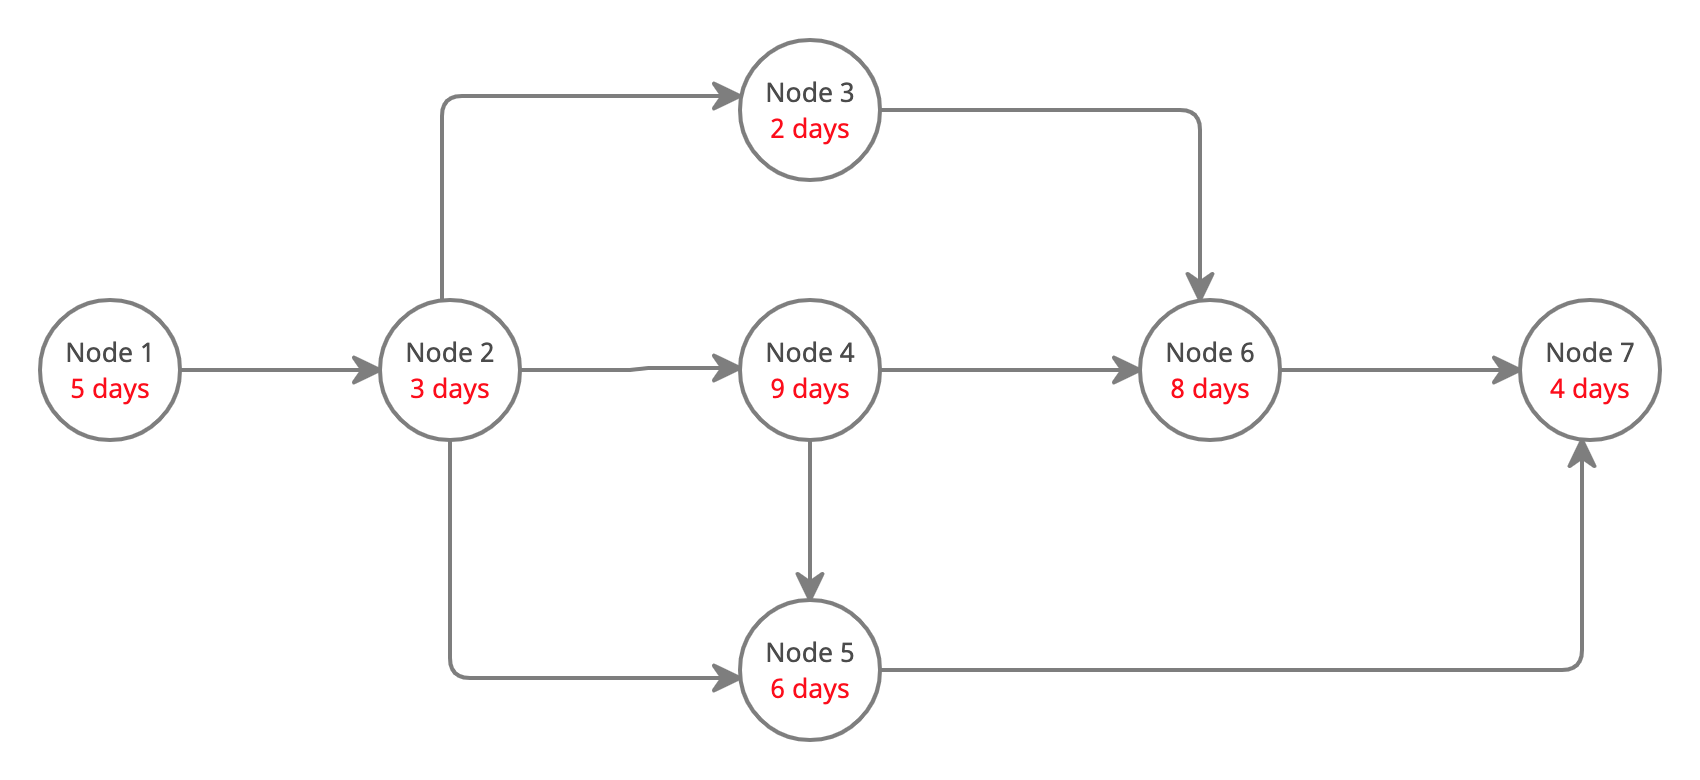
\includegraphics[width=130mm]{activity_graph.png}
  \caption{Sample activity node diagram}
  \label{node pairs}
\end{figure}

Each node pair has to be represented in order to ensure accurate results when accessing the \verb+.duration.days+ property or even while calling the \linebreak\verb+.get_critical_path()+. Repitions are ignored. For \autoref{node pairs}, the relevant node pairs are 

\begin{itemize}
  \item node1, node2
  \item node2, node3
  \item node3, node6
  \item node6, node7
  \item node2, node4
  \item node4, node6
  \item node2, node5
  \item node4, node5
  \item node5, node7
\end{itemize}


\subsection{The Project class}
The project class serves as a demonstration as to how the other class objects can be managed under a common umbrella. It provides an interface for interacting with other objects and performing operations on them.

\begin{lstlisting}
  class Project(project_charter):
      # methods
      method create_deliverable(self, deliverable_name)
      method add_deliverable(self, deliverable: Deliverable)
      method accept_deliverable(self, deliverable: Deliverable)
      method reject_deliverable(self, deliverable: Deliverable)
      method add_new_project_risk(self, risk)

      # properties
      property deliverables
      property project_risks
      property project_charter
      property stakeholders
      property project_governance
\end{lstlisting}

\verb+.create_deliverable()+ method take an argument, \verb+deliverable_name+ and returns an object of type \verb+Deliverable+. It also calls the method \verb+.add_deliverable()+ with the newly created \verb+Deliverable+ object as the only argument.

\verb+.accept_deliverable()+ and \verb+.reject_deliverable()+ are light wrappers around the Deliverable objects and serve to mark the deliverable objects as accepted or rejected using the methods \verb+.mark_as_accepted()+ and \verb+.mark_as_rejected()+ which the deliverable objects provides themselves.

\begin{lstlisting}
  class Project:

      ...

      def accept_deliverable(self, deliverable: Deliverable):
          assert deliverable in self._deliverables, "Deliverable does not exist within the current project"
          deliverable.mark_as_accepted()

      def reject_deliverable(self, deliverable: Deliverable):
          assert deliverable in self._deliverables, "Deliverable does not exist within the current project"
          deliverable.mark_as_rejected()
\end{lstlisting}


  \chapter{Testing}
  \section{What is Testing}
In general, testing is finding out how well something works. Software testing is the act of examining the artifacts and the behavior of the software under test by validation and verification \cite{wikipedia-testing}.

There are several types of tests that can be carried out on a software but for the sake of this thesis project, all emphasis will be on unit test.

\section{What is unit testing}
Unit testing is a type of software testing where individual units or components of a software are tested. The goal is to ensure that each unit of software code works as intended. Unit test is carried out by developers throughout the development (coding) phase of an application. Unit tests are used to isolate a part of code and ensure that it is correct. Any singular function, method, process, module, or object might be considered a unit.

Unit testing ensures that all code meets quality standards before it’s deployed. This ensures a reliable engineering environment where quality is paramount. Over the course of the product development life cycle, unit testing saves time and money, and helps developers write better code, more efficiently. It offers a wide variety of advantages but a few has been listed below:

\begin{itemize}
  \item \textbf{Bugs are found easily and quicker:} Code that is covered by tests is more dependable than code that is not. If a future modification breaks something in the code, developers will be able to quickly pinpoint the source of the problem rather than having to sift through a large codebase.
  \item \textbf{Unit testing provides documentation:} Unit tests are a type of living product documentation. Developers can use unit tests to acquire a basic overview of the logic of a module and the system as a whole in order to figure out what functionality is offered by one module vs another. Unit test cases are indications that provide information about whether a software component is being used correctly or incorrectly. As a result, these examples serve as excellent documentation for these indicators.
  \item \textbf{Modularity:} Thanks to the modular nature of the unit testing, parts of a project can be tested without waiting for others to be completed.
\end{itemize}


\section{Testing the library}
Each module and each function down to each line of code was tested yielding a 100\% test coverage. Pytest, a popular Python testing library, was used to accomplish the test. A sample test case is included.

\begin{lstlisting}
  from project import Project
  from unittest.mock import Mock
  from project.governance import ProjectGovernance


  def test_Project(project: Project):
      assert str(project) == "Fake Project"
      assert isinstance(project.project_charter, Mock)
      assert hasattr(project.project_charter, "project_stakeholders")
      assert hasattr(project.project_charter, "project_title")
      assert isinstance(project.project_governance, ProjectGovernance)
      assert project.deliverables == []
      assert project.project_risks == []
\end{lstlisting}

The test cases are enforced through a series of \verb+assert+ statements

These tests were configured to run automatically on GitHub using Github Actions whenever there's a new push to the repository. The configuration is in a \verb+.yaml+ file format.

\pagebreak

\begin{lstlisting}
  name: Test

  on:
    push:
    pull_request:
      branches:
        - master

  jobs:
    test:
      runs-on: ubuntu-latest

      steps:
        - name: Check Out
          uses: actions/checkout@v2

        - name: Get Branch Name
          run: echo "BRANCH=$(echo ${GITHUB_REF##*/})" >> $GITHUB_ENV

        - name: Install requirements, run tests with make and write coverage
          run: make testall

        - name: Get Coverage for badge
          run: echo "COVERAGE=$(cat coverage.json | jq .totals.percent_covered)%" >> $GITHUB_ENV

        - name: Create Badge
          uses: schneegans/dynamic-badges-action@v1.1.0
          with:
            auth: ${{ secrets.GIST_SECRET }}
            gistID: a1817190b63b0cd8f551cb3ec2ab6524
            filename: ${{ github.event.repository.name }}_${{ env.BRANCH }}_coverage.json
            label: Code Coverage
            message: ${{ env.COVERAGE }}
            color: green
            namedLogo: GitHub Actions

\end{lstlisting}

The source code and tests in their entirety are in the \autoref{appendix:sourcecode} and \autoref{appendix:unittest} section respectively


  \chapter{Conclusion}
  \section{Outcomes}The thesis's outcome is stated in light of the thesis's goal and scope, which were established at the beginning.

The main purpose of this thesis was to develop a project management library. It was designed to provide the basic functionality that will be needed when developing a thesis management web application but can be also be adapted for other purposes. Extensive unit tests have also been written to ensure that when future functionalities are implemented, old ones don't break. These tests have been configured to run automatedly in Github hosted linux runners. The result of this test is attached to a badge on the README.md on the repository to give library users a quick insight about the health of the source code.


\section{Future Improvements}
\begin{itemize}
  \item Right now, it's just a library and haven't been used in any MVP yet. Utilizing and integrating this library in real world applications will lead to improvement as some bugs that might have slipped through the unit testing procedure might eventually be discovered and fixed.
  \item Integrate a static tool checker like mypy. Python is a dynamically typed language meaning that variables that point to objects can be assigned different data types during their lifetime. Integrating mypy will reduce errors stemming from wrong data type assignment.
  \item Loosely couple modules to promote independent use. Some modules require other modules. For instance, the \verb+governance+ module requires a \verb+Stakeholder+ object from the \verb+project_stakeholder+ module. This creates interdependence making using one and not the other impossible. It will be beneficial to conduct an analysis and implement design patterns to solve the concern.
\end{itemize}

  \cleardoublepage
  \phantomsection
  \addcontentsline{toc}{chapter}{References}
  \bibliographystyle{unsrt}
  \renewcommand{\bibname}{References}
  \bibliography{references}

  \appendix

  \chapter{Source code}\label{appendix:sourcecode}
  \UseRawInputEncoding

\section{src/project/\_\_init\_\_.py}
\lstinputlisting{library/src/project/__init__.py}

\pagebreak

\section{src/project/deliverables/\_\_init\_\_.py}
\lstinputlisting{library/src/project/deliverables/__init__.py}

\pagebreak

\section{src/project/governance/\_\_init\_\_.py}
\lstinputlisting{library/src/project/governance/__init__.py}

\pagebreak

\section{src/project/project\_charter/\_\_init\_\_.py}
\lstinputlisting{library/src/project/project_charter/__init__.py}

\pagebreak

\section{src/project/project\_stakeholder/helpers.py}
\lstinputlisting{library/src/project/project_stakeholder/helpers.py}

\pagebreak

\section{src/project/project\_stakeholder/\_\_init\_\_.py}
\lstinputlisting{library/src/project/project_stakeholder/__init__.py}

\pagebreak

\section{src/project/risks/helpers.py}
\lstinputlisting{library/src/project/risks/helpers.py}

\pagebreak

\section{src/project/risks/\_\_init\_\_.py}
\lstinputlisting{library/src/project/risks/__init__.py}

\pagebreak

\section{src/project/wbs/\_\_init\_\_.py}
\lstinputlisting{library/src/project/wbs/__init__.py}

\pagebreak

\section{src/project/wbs\_item/\_\_init\_\_.py}
\lstinputlisting{library/src/project/wbs_item/__init__.py}

\pagebreak

\section{src/utils/\_\_init\_\_.py}
\lstinputlisting{library/src/utils/__init__.py}

\pagebreak

\section{src/utils/generic\_document.py}
\lstinputlisting{library/src/utils/generic_document.py}

\pagebreak

\section{src/utils/stakeholder.py}
\lstinputlisting{library/src/utils/stakeholder.py}

  \chapter{Unit test code}\label{appendix:unittest}
  \section{tests/factories.py}
\lstinputlisting{library/tests/factories.py}

\pagebreak

\section{tests/faker.py}
\lstinputlisting{library/tests/faker.py}

\pagebreak

\section{tests/test\_project/test\_deliverables.py}
\lstinputlisting{library/tests/test_project/test_deliverables.py}

\pagebreak

\section{tests/test\_project/test\_governance.py}
\lstinputlisting{library/tests/test_project/test_governance.py}

\pagebreak

\section{tests/test\_project/test\_project\_charter.py}
\lstinputlisting{library/tests/test_project/test_project_charter.py}

\pagebreak

\section{tests/test\_project/test\_project\_stakeholder.py}
\lstinputlisting{library/tests/test_project/test_project_stakeholder.py}

\pagebreak

\section{tests/test\_project/test\_project.py}
\lstinputlisting{library/tests/test_project/test_project.py}

\pagebreak

\section{tests/test\_project/test\_risks.py}
\lstinputlisting{library/tests/test_project/test_risks.py}

\pagebreak

\section{tests/test\_project/test\_wbs\_item.py}
\lstinputlisting{library/tests/test_project/test_wbs_item.py}

\pagebreak

\section{tests/test\_project/test\_wbs.py}
\lstinputlisting{library/tests/test_project/test_wbs.py}

\pagebreak

\section{tests/test\_utils/test\_generic\_document.py}
\lstinputlisting{library/tests/test_utils/test_generic_document.py}

\pagebreak

\section{tests/test\_utils/test\_stakeholder.py}
\lstinputlisting{library/tests/test_utils/test_stakeholder.py}


\end{document}